\chapter{Rigorous procedures to include multiple fragment topologies in
electronic structure for dynamics and potential surface calculations}

\section{Set theoretic measures for dividing a molecular system}

\label{dynafrag}
To clarify the problem in general terms, in Figure
\ref{dirichlet-tessalation}(b), we represent a fragmented version of
a protonated water-wire ($(H_{2}O)_{12}H^{+}$) presented in Figure
\ref{dirichlet-tessalation}(a). Molecular entities contained within each
ellipse are called primary fragments. For example, Figure
\ref{dirichlet-tessalation}(b) contains either dimers ($(H_{2}O)_{2}$)
or protonated dimers ($(H_{2}O)_{2}H^{+}$) as primary fragments. The
molecular entities present in the intersection region of ellipses
are called derivative fragments. Hence Figure \ref{dirichlet-tessalation} (b)
contains either water ($H_{2}O$) or hydronium ion ($H_{3}O^{+}$) as
derivative fragments. Figure \ref{dirichlet-tessalation} is presented
here purely for illustrative purposes and more general fragmentation
schemes may be visualized, and are in fact routinely used
cite{Tim-paper}TOBECHANGED.

The image in Figure \ref{dirichlet-tessalation}(b) is algebraically
translated using the set-theoretic principle of inclusion exclusion
(PIE)\cite{pie} where each ellipse and each of their overlapping
regions carry energy correction to the overall system. The associated
inclusion-exclusion principle based generalization of the ONIOM method
\cite{oniom} presented in Refs.\cite{fragAIMD,fragAIMD-elbo,fragAIMD-CC}
has the mathematical form

\begin{align}
E^{PIE-ONIOM} \approx & ~E^{level,0}(0) + \sum^n_{i=1}{\cal S}(i) - \sum_{1<=i<j<=n}{\cal S}(i\cap
j)+\sum_{1<=i<j<k<=n}{\cal S}(i\cap j\cap k)- \cdots + \nonumber \\ & (-1)^{n-1}\sum {\cal
  S}(1\cap \cdots \cap n).
\label{eq:pie-oniom}
\end{align}

\noindent where $E^{level,0}(0)$ is the energy corresponding to the full system
in Figure \ref{dirichlet-tessalation}(b) at some predefined lower level
of theory, whereas

\begin{equation}
{\cal S}\left(i\right) = E^{level,1}\left(i \right)-E^{level,0}\left(i\right),
\label{oniombasic-2}
\end{equation}

\noindent represents a correction term arising from each molecular fragment
depicted with an ellipse (represented using the index $i$ and $j$) or each
molecular fragment with overlapping regions (represented using the notation
$i\cap j$), and so on. Thus, the fragmentation scheme in Figure \ref{dirichlet-tessalation}
(b) leads to a hierarchy of fragments to be used to compute energies and forces.
It should be noted that the PIE expression takes care of over counted regions
in the fragmentation calculations. Overlaps used in the fragmentation allows
us to include most of the important interactions of the system. Important
interactions are generally kept intact during fragmentation schemes. Energy
correction terms in the PIE expression are included by calculating both high
as well as low level of theory calculation on primary and derivative
fragments. When a bond is broken in a fragmentation scheme, link atoms are
added to both the fragments created this way. Generally, hydrogen atom is
chosen to be the link atom but it has been shown \cite{qwaimdqmmm} that other
atoms or a group of atoms may also be used to match the electronegativities.
The bond distances for the link atoms attached are calculated by using
a scaling parameter that depends on the nature of bond cut during fragmentation
\cite{dapprich1999new}. Full system calculation performed at lower level
includes long range interactions in the system. After we add these correction
terms to the long range interactions, the accuracy of the method turns out
to be similar to the higher level of theory calculations. These high and low
level of theories can be two different theories for example, MP2
and Density Functional Theory (DFT) or two
different basis sets used with a same level of theory.

\section{Challenges for AIMD and potential surface calculations}
Despite the progress highlighted above, critical challenges remain in
both fragment based dynamics and in potential energy surface calculations.
For example, molecular fragmentation is a dynamical phenomenon that in
general changes with time during dynamics. While one expects such effects for
the case of strongly hydrogen bonded systems, such as water-clusters, where
excursions of the shared proton along the hydrogen-bond donor-acceptor region may
cause a change in connectivity and hence the fragment topology\footnote{The terms
``fragment topology'' or ``topology'' are used throughout this report and
both of them refer to the definition of fragments  used during fragment based
electronic structure calculations.}, the problem is much more general and may
include cases such as solvation effects in peptide
fragments and other organic molecules of significance in atmospheric chemistry
\cite{isobut2D-water}. For the case of strongly hydrogen bonded systems,
such as water-wires that are found in many biological\cite{qmmmadmp,Roux,Sagnella,
pomesRoux1, nagle1978molecular, baciou1995interruption, takeshita2014x,
chamberlin2015mapping, sasaki2006voltage, ramsey2006voltage} and materials chemistry
problems\cite{mashl2003anomalously, si2011selective, mann2003water}, and other
hydrogen bonded chains \cite{Guo}, the excursion of the shared protons may be
correlated, much like the case of secondary isotope effects note in
Ref. \cite{SLO-rare-isotopes}, and this may result in multiple bonding
configurations to contribute simultaneously.

In Figure \ref{chap1fig1}, we present an illustration of this problem where the
evolution of total energy for a solvated Zundel system is presented from a
frag-BOMD simulation. The singular hops in total energy are time-steps
where the fragment topology changed due to geometric
changes. Two of the many fragmentation topologies are shown in Figure
\ref{chap1fig1}. It can be seen that the proton in the centre of solvated Zundel
cation system is present in all the primary fragments shown in red on the left
side, but this is not the case in the primary fragments shown in blue on the
right side of Figure \ref{chap1fig1}.

\begin{figure}[H]
  \begin{center}
    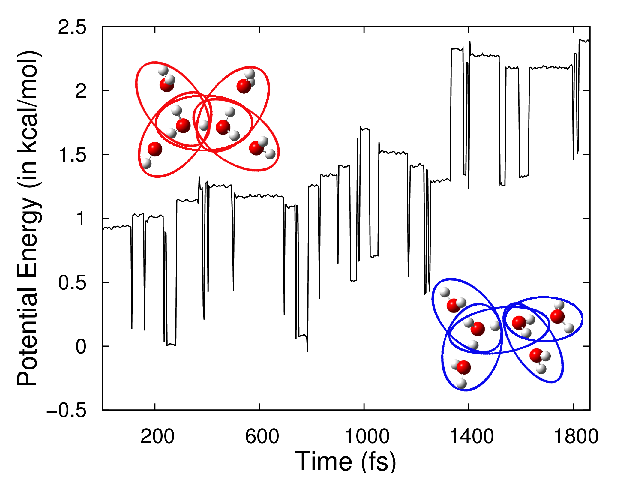
\includegraphics[width=0.6\textwidth]{figures/bomdEnergy.eps}
    \caption{\label{chap1fig1} The evolution of electronic potential energy during a
    fragment-based BOMD calculations for the solvated Zundel cation is shown. The singular
    hops in the potential are due to change in fragment description, two of which
    are presented in the figure with ellipses describing fragments. Note that the
    figure with ellipses marked in blue has a different fragment description as
    compared to that in red.}
  \end{center}
\end{figure}

In Figure \ref{chap1fig2} and Figure \ref{chap1fig3}, we provide an example for
the change in fragment topology
during reduced dimensional potential energy surfaces (PES) computed to account for
nuclear quantum effects. The system involved is a water-wire shown on top of Figure
\ref{chap1fig2}.

\begin{figure*}[t!]
    \centering
    \begin{subfigure}[t]{0.5\textwidth}
        \centering
        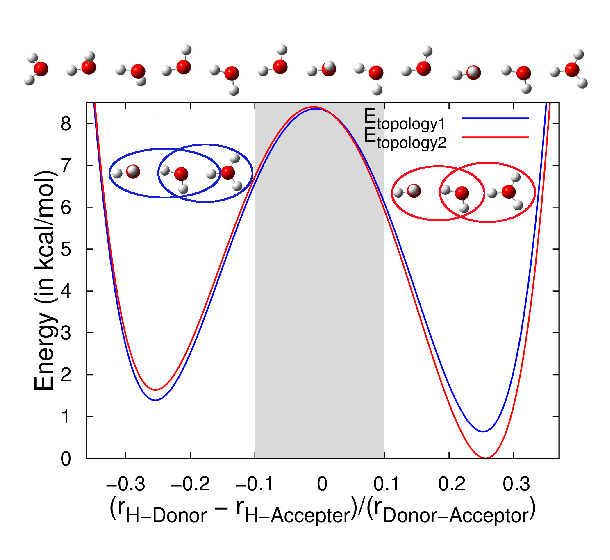
\includegraphics[width=0.9\textwidth]{figures/graph1all.eps}
        \caption{\label{chap1fig2}}
    \end{subfigure}%
    ~
    \begin{subfigure}[t]{0.5\textwidth}
        \centering
        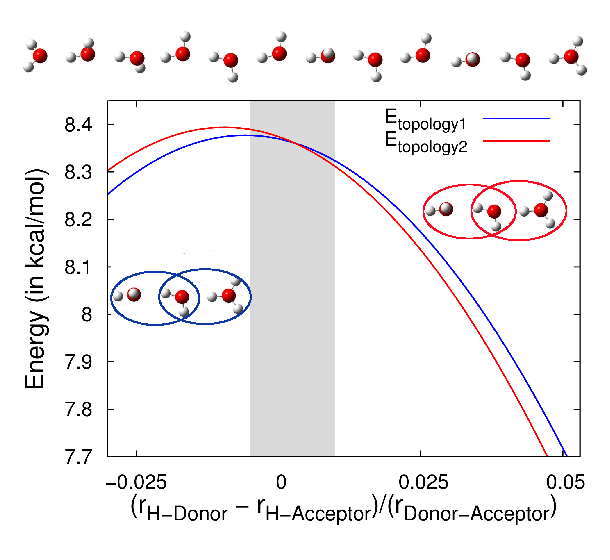
\includegraphics[width=0.9\textwidth]{figures/reZoomedInWithoutCTM.eps}
        \caption{\label{chap1fig3}}
    \end{subfigure}
    \caption{ A potential surface for the shared proton in a water-wire system is
    shown in Figure \ref{chap1fig2}, the fact that the fragments in red have different
    identities as compared to the fragments in blue, leads to two different
    surfaces. Figure \ref{chap1fig3} provides an enhanced version of the differences.}
\end{figure*}

Such systems are commonly found in many biological problems \cite{qmmmadmp,Roux,Sagnella,
Guo,Agre,Takata,Kandori} and materials chemistry problems \cite{mashl2003anomalously,
si2011selective, mann2003water}, but are also of fundamental significance to aqueous
reactive chemistry. The potential surfaces are \textbf{significantly TO BE CHANGED}
different depending
on which fragment topology is used,two of which are shown in Figure \ref{chap1fig2}.
It is critical to note
that during an adaptive fragmentation process, required in AIMD and in PES calculations,
many such topologies can automatically appear and it is critical to develop an adaptive
approach that can treat such more complex chemical phenomena and this is the
underlying goal for this report. Furthermore, such differences in potential surfaces may
occur in $3N$-dimensions and hence, the method developed here works for arbitrary dimensions
with arbitrary number of topologies.

\section{Formal constructs for a multi-topology formalism}
Let us now consider the situation where the energy of the system is not accurately
described by a single fragmentation protocol. This could for example be the case for
a reactive system close to its transition state where the system maintains features
from both reactant and product topologies. Alternatively for water cluster, or a molecule,
such as a peptide fragment, solvated in a protic (including excess protons and excess
hydroxides) solvent such as water, depending upon the structure and position of the
heavy atoms in the system, the position of protons is labile and hence the connectivity
and fragmentation protocols may not be unique. Certainly, this would be a very significant
during dynamics and during potential energy surface calculations for degrees of freedom
pertaining to specific nuclear degrees of freedom (such as the excess proton or excess
hydroxide delocalization). Another complex case could deal with large scale changes in
protein structure, but this problem is not explicitly dealt with here. In all cases, it
is perhaps necessary to think of the overall energy of the system as a probabilistic sum
over multiple fragmentation protocols or multiple topological networks and hence:

\begin{equation}
\left\langle E \right\rangle = \sum_{\alpha=0}^N p_\alpha * E^{PIE-ONIOM}_\alpha
\label{aveE}
\end{equation}
where $p_\alpha$ is the probability corresponding to topology $\alpha$, with energy
$E^{PIE-ONIOM}_\alpha$. Note that topology $\alpha$ represents a certain fragmentation
protocol such as that in Figure \ref{dirichlet-tessalation}(b). A different topology,
$\beta$, has a different fragmentation and hence different energy and gradients. 

How are the family of $\left\{p_\alpha\right\}$-values to be computed? 
There are three directions that we discuss in this report: 
\begin{itemize}
\item[(a)] In probably the most straight-forward implementation, we cast this
multiple-topology scheme into a "Hamiltonian"-formalism, where the off-diagonal
elements include hopping probabilities from one topology to the other; the
diagonal elements include energy contributions from each topological description
of the system. This particular formalism is completely benchmarked in this report
and presented in Chapter 3, with its development discussed in detail in later
parts of Chapter 2.
\item[(b)] In future work (Chapter 4), we re-interpret approach (a) above in a
manner akin to non-adiabatic dynamics, and invoke Tully's surface hopping
\cite{tully1971trajectory} to construct a "stochastic-Hamiltonian" scheme to
construct classical dynamics across multiple "surfaces". At this stage we will
explore other measure such as Landau-Zener-hopping and Pechukas theory, but it
is critical to state that our re-interpretation of this problem in the
non-adiabatic sense is deeply enriching towards the development of new
computational methods in this case.
\item[(c)] Our eventual goal is to construct wavepacket dynamics on these
multiple surfaces and that will also be considered as part of future work.
\end{itemize}
An overarching treatment that encompasses all three ideas above may be
obtained by considering multi-topology dynamics using Feynman path-integrals
\cite{feynman2010quantum} which is what we do next. 

Consider $N+1$ $\it{neighboring}$  topologies numbered
$\alpha=0,\cdots,N$.  Without loss of generality, we assume that the current molecular structure 
in dynamics or in a potential surface calculation belongs to topology $0$. Let
$p_{\alpha \rightarrow \beta}$ be the
probability of a direct hop from topology $\alpha \rightarrow \beta$. In that case, the
net probability of a hop from $0 \rightarrow \alpha$ may be expressed as discrete sum over
paths in fragment-topological space given by
\begin{equation}
p_\alpha = p_{0 \rightarrow \alpha} + \sum_{\beta}{}^{\prime} ~p_{0 \rightarrow \beta} p_{\beta \rightarrow \alpha} +
\sum_{\beta,\gamma}{}^\prime ~p_{0 \rightarrow \beta} p_{\beta \rightarrow \gamma} p_{\gamma \rightarrow \alpha} +
\sum_{\beta,\gamma,\delta}{}^\prime ~p_{0 \rightarrow \beta} p_{\beta \rightarrow \gamma} p_{\gamma \rightarrow \delta} p_{\delta
  \rightarrow \alpha} +
\cdots
\label{pJ}
\end{equation}
where the superscript prime following the summation indicates that the
summation variables cannot be equal to each other, nor can these be equal to $0$ or
$\alpha$. By definition, the probabilities must add
up to one, and hence, the probability of remaining in topology $0$ is simply 
\begin{equation}
p_0 = 1 - \sum_\alpha p_\alpha
\label{p0}
\end{equation}
Note also that for situations where the topology change is sequential, that
is there is only one other energetically comparable topology available in
addition to the current topology, $p_J \equiv p_{0 \rightarrow J}$.
Furthermore, $p_\alpha \equiv p_\alpha({\bf R})$, that is the probability of choosing a
given topology is a function of the nuclear coordinates and is hence a
time-dependent factor to be computed during dynamics. We interpret the topological
states as diabatic states to provide the connections discussed above and in further
details in following sections and chapters.


\section{A pseudo-Hamiltonian formalism that allows continuous morphing across topologies}
{\label{CTMSection}}
We define the network topologies as our diabatic states and propose a general method
for interpolation across an arbitrary number of such states, in the sense of Eq. \ref{aveE}.
Say, there are n topological networks, or fragmentation protocols, encountered during a dynamics
or reduced dimensional
potential energy surface calculation. We further assume that, the fragmentation based potential
energies corresponding to these networks are given by the set of energies
$\left\{ E_\alpha^{PIE-ONIOM} \right\}$, where $\alpha = 1 \cdots n$. 
A "Hamiltonian" matrix $M_{n \times n}$ is formed using the following set of rules and helps
determine the "multi-configurational" coefficients in Eq. \ref{aveE}.
\begin{enumerate}
  \item The diagonal elements are $M_{ii} = E^{PIE-ONIOM}_{i}$, where $i \in {1, 2,.., n}$.
  \item If the fragmentation protocols don't change directly from i to j then $M_{i,j} = M_{j,i} = 0$.
  \item If the fragmentation protocols change directly from i to j then a neighbourhood
  is defined within a reduced unit interval $(t_{ij}^{0},t_{ij}^{1})$ containing the hop. These
  "reduced-units" may be a reaction coordinate in a reactive process, reduced dimensional degrees
  of freedom that influence a potential energy scan, or simply a time-interval during a classical
  dynamics process. Hence there are two cases:
  \begin{enumerate}
    \item if t $\not\in$ $(t_{ij}^{0},t_{ij}^{1})$, then $M_{i,j} = M_{j,i} = 0$,
    \item if t $\in$ $(t_{ij}^{0},t_{ij}^{1})$, then $M_{i,j}$ is given by
    \begin{equation}
    M_{ij}^{2} = \it f(x_{ij})(f(x_{ij})-1)(E^{PIE-ONIOM}_i-E^{PIE-ONIOM}_j)^{2}
    \label{offDiagEquation}
    \end{equation}
    \noindent where, function $\it f(x_{ij})$ is chosen as smooth Heaviside function with a specific parameters
    \begin{equation}
    f(x_{ij}) = a(erf(b(x_{ij}-c)) + 1)
    \label{fx_function}
    \end{equation}
    \noindent where a, b and c are vertical height, width and right shift parameters
    respectively. These parameters a, b, and c are chosen as 0.5, 5 and 0.5 respectively
    such that $x_{ij} \in$ (0,1) $\rightarrow f(x_{ij}) \in (0,1)$.

    For t $\in$ $(t_{ij}^{0},t_{ij}^{1})$, $x_{ij}$ is defined as
    \begin{equation}
    x_{ij}(t) = \frac{t-t_{ij}^{0}}{t_{ij}^{1}-t_{ij}^{0}}\,
    \label{paramEquation}
    \end{equation}
  \end{enumerate}
\end{enumerate}

The smooth Heaviside function will tend to a step function as $b \to \infty$. Hence,
shifting at the seam is just a special case of this interpolation. This method
allows the users to utilize a function with their choice of smoothness. More details on
$f(x)$ are given in Appendix C.

\noindent At the end the complex eigenvalue solver is used to calculate all the eigenvalues and
the lowest eigenvalue is chosen to be the ground state potential energy of the system. The choice
for the function $M_{ij}$ and $f(x)$ is inspired by the fact that we need $M_{ij}$ to go to zero
as x $\rightarrow$ 0 or 1.

It can be clearly seen from the Eq. \ref{offDiagEquation} that all the off-diagonal elements
will be purely imaginary.
For a set of energies $\left\{ E_\alpha^{PIE-ONIOM} \right\}$, where
$\alpha = 1 \cdots n$, the choice of a Hermitian matrix $M$ leads to a lowest eigenvalue of $M$
that doesn't lie in between the two smallest energies from the set. Only the purely imaginary
off-diagonal containing symmetric matrices can lead to a lowest eigenvalue lying in between the
two smallest energies from the set. Critical aspects associated with this are discussed
in Appendix A.

We name this method of interpolation as $\bf{Continuous ~Topology ~Morphing ~(CTM)}$ and for the
rest of this report the abbreviation CTM will added to quantities related interpolated results.


\section{Computational efficiency for potential surface calculations}
Due to a large number of electronic structure calculations, computational efficiency in creating
potential energy surfaces is always point of consideration. For each point on the grid, fragment
based electronic structure is used to reduce the computational cost. Parallel computing implementation
of these fragment's potential energy calculations lead to a reduction in computational cost. It
turn out that this cost can further be reduced for most of the reduced dimensional potential energy
surface calculations. Only a few fragments among all, actually change during a potential energy
scan. Hence, a scheme was devised to only perform the minimum number of electronic structure
calculations required in the whole process. This scheme lead to a huge computational gain. More
details about it are given in Appendix B.


A brief discussion about the other methods developed in the similar domains are discussed
below. These methods cover a wide range of scientific areas and hence show how vast is
the domain of these kind of problems is.

\section{NEEDS TO BE MODIFIED Other methods developed to solve similar problems}
Arieh Warshel and Robert M. Wiess developed empirical valence bond (EVB) method
for calculating potential energy surfaces of reactions that happen in solution phase or
in enzymes \cite{jacs102.6218}.
%Main focus of this method was to study ionic bond breaking reactions, proton-
%transfer and general acid catalysis reactions. Ionic and covalent states were used in a
%2 by 2 EVB Hamiltonian. Potential energy values corresponding to the ionic and covalent
%states were used as diagonal elements and the off-diagonal element was calculated by
%using experimental ground-state bond energy. Analytical expression was used to get the
%ground state eigenvalues. Heterolytic cleavage of the glycosidic bond of a disaccharide
%was the reaction studied in the publication \cite{jacs102.6218}.
Udo W. Schmitt and Gregory A. Voth developed a multi-state empirical valence bond
model (MS-EVB) \cite{schmitt1998multistate} to simulate proton transport in water. This
model was parametrized for selected $H_3O^+.(H_3O)_N$ systems to get geometric and
energetic quantities \cite{luz1964activation}.
% This method utilized a geometric based criteria to come up with all
%the possible states within a system and reported to have around 6 to 10 states for their
%systems. Their off-diagonal element was calculated by product of an additive potential
%and a geometric function chosen for three parameters such as $O-O$ distance, asymmetric
%stretch coordinate and bend angle corresponding to $H_5O_2^+$. The finally the proton
%hopping rate (0.25 $ps^{-1}$) was compared to the experimental result
%(0.7 $ps^{-1}$ ~\cite{luz1964activation}).
Rode and co-workers developed \cite{kerdcharoen1996qm, hofer2005structure,
schwenk2003structure} a force smoothening scheme called hot spot method for QM/MM based
MD simulations.
%They partitioned the whole molecular system including the solvent into
%three regions active region, buffer region and environmental region respectively. A
%smoothing function based on was used to interpolate the forces of only on the
%atoms/molecules present in the buffer region. Potential energy was not interpolated
%in this method. This method worked well while performing canonical ensemble base MD
%simulations using the Berendsen algorithm \cite{berendsen1984molecular} but it lacked
%energy and momentum conservation. 
Kerdcharoen and Morokuma developed the ONIOM-XS method which was also based
on the based on a smoothing function but also included the smoothing the potential
along with the forces on the atoms/molecules present in the buffer region.
%This method works well if only on group is present in the buffer region but fails to
%conserve energy in an NVE ensemble base MD simulation if more than one groups are
%present in the buffer region. To solve the problem of multiple groups (atoms/molecules)
%being in the buffer region, 
Morokuma and co-workers also developed adaptive partitioning based methods, Permuted AP
method and Sorted AP method. Both of these conserve energy and forces.
% Permuted AP method scales as $2^N$ but Sorted
%AP method scales as N only, where N is number of groups present in the buffer region.
%Both of these methods use ideas very similar to multi-body expansion schemes.

\newpage

